% ============================================================
%  Chapter 5: Results
% ============================================================

\chapter{Results}
\label{ch:results}

This chapter presents the experimental results of \modnet{} on the
six benchmark tasks described in Chapter~\ref{ch:experiments}.
We report quantitative outcomes, qualitative analysis of the evolved
structures, and a detailed examination of one case (Parity-6) in
which the network failed to reach the success threshold.

% ------------------------------------------------------------
\section{Overview}
\label{sec:overview}
\label{sec:results-overview}
% ------------------------------------------------------------

Table~\ref{tab:main-results} summarizes the outcome of all six
experiments. Four of the six tasks reached their success threshold:
XOR2 and Parity4 at $100\%$ accuracy, and sin2pi and circle at RMSE
below $0.05$. Two tasks fell short: Parity6 reached $93.8\%$ accuracy,
and sin4pi reached RMSE $0.073$, above the $0.10$ success threshold.

\begin{table}[h]
  \centering
  \small
  \caption{Summary of experimental results. All tasks use the same
    architecture and evolutionary algorithm; only the number of time
    steps $T$ and the encoding differ.}
  \label{tab:main-results}
  \begin{tabular}{llrrrrrr}
    \toprule
    \textbf{Task} & \textbf{Metric} & \textbf{Result} & $N$
      & $E$ & $Q$ & $R$ & \textbf{Time (s)} \\
    \midrule
    XOR2      & Accuracy   & $\mathbf{100.0\%}$     &  8 &  17 & 14 & 2 &  0.4 \\
    Parity4   & Accuracy   & $\mathbf{100.0\%}$     & 12 &  74 & 45 & 9 &  4.2 \\
    Parity6   & Accuracy   & $93.8\%$               & 10 &  67 & 50 & 8 & 27.2 \\
    sin2pi    & RMSE       & $\mathbf{0.0412}$      & 30 & 296 & 218 & 13 & 38.3 \\
    sin4pi    & RMSE       & $0.0729$               & 19 & 168 & 120 & 7 & 27.9 \\
    Circle    & RMSE       & $\mathbf{0.0222}$      & 29 & 237 & 180 & 9 & 12.0 \\
    \bottomrule
  \end{tabular}
  \vspace{0.3em}
  \par\footnotesize{$N$: nodes in final network. $E$: active connections.
  $Q$: cross-module connections. $R$: recurrent self-loops.
  Numbers in bold indicate that the task met its success threshold.}
\end{table}

Three observations follow immediately from Table~\ref{tab:main-results}.
First, the architecture is capable of solving tasks that require
nonlinear computation: XOR and parity are both provably impossible for
a single linear threshold unit \citep{minsky1969perceptrons}. Second,
the same architecture, with no task-specific modifications, handles
both Boolean and continuous regression problems. Third, the evolved
networks are small: no task required more than 30 nodes, and the
simplest task (XOR) required only 8.

% ------------------------------------------------------------
\section{Boolean Function Learning}
\label{sec:results-boolean}
% ------------------------------------------------------------

\subsection{XOR (2-bit)}
\label{sec:results-xor}
% ------------------------------------------------------------

\modnet{} solved XOR in 32 generations, using only 8 nodes and 17
active connections (Figure~\ref{fig:xor2-network}). The final network
has module sizes $[2, 3, 2, 1]$ and 14 cross-module connections, with
2 recurrent self-loops.

\begin{figure}[h]
  \centering
  
\includegraphics[width=0.7\textwidth]{xor2/best.pdf}
  \caption{The final network evolved for the XOR task. Nodes are
    colored by module (see Chapter~\ref{ch:method} for the color
    legend). Cross-module connections dominate: 14 of the 17 active
    connections cross module boundaries. The network uses only 27\% of
    the available connections (17 of 64), and contains 2 recurrent
    self-loops.}
  \label{fig:xor2-network}
\end{figure}

The learning curve for XOR (Figure~\ref{fig:xor2-curve}) is
characteristic of the search behaviour across all tasks: an initial
plateau at $f = -0.25$ (the fitness value corresponding to always
predicting $0$), followed by a rapid jump to $f = 0$ once a
sufficiently expressive topology is discovered.

\begin{figure}[h]
  \centering
  
\includegraphics[width=0.7\textwidth]{xor2/curve.pdf}
  \caption{Learning curve for XOR. The fitness improves from $-0.25$
    (chance level) to $0$ (perfect accuracy) in 32 generations. The
    rapid jump indicates that once a topology capable of computing
    XOR is found, it is immediately perfected.}
  \label{fig:xor2-curve}
\end{figure}

The complete input--output mapping is shown in
Table~\ref{tab:xor2-samples}. All four input combinations are
classified correctly.

\begin{table}[h]
  \centering
  \small
  \caption{Input--output mapping for the evolved XOR network.}
  \label{tab:xor2-samples}
  \begin{tabular}{cc|c}
    \toprule
    \textbf{Input $a$} & \textbf{Input $b$} & \textbf{Output} \\
    \midrule
    0 & 0 & 0 \\
    0 & 1 & 1 \\
    1 & 0 & 1 \\
    1 & 1 & 0 \\
    \bottomrule
  \end{tabular}
\end{table}

\subsection{Parity (4-bit)}
\label{sec:results-parity4}
% ------------------------------------------------------------

Parity-4 was solved exactly ($100\%$ accuracy) in 320 generations
using 12 nodes and 74 active connections (Figure~\ref{fig:parity4-network}).
The final network has module sizes $[5, 3, 3, 1]$, with 45 cross-module
connections and 9 recurrent self-loops. All 16 input combinations are
classified correctly (Table~\ref{tab:parity4-samples}).

\begin{figure}[h]
  \centering
  
\includegraphics[width=0.7\textwidth]{parity4/best.pdf}
  \caption{The final network evolved for 4-bit parity. The output
    module (right) contains a single node, which receives input from
    all three earlier modules. Recurrence is present in 9 of the 12
    nodes, indicating that the network uses temporal computation
    extensively.}
  \label{fig:parity4-network}
\end{figure}

\begin{figure}[h]
  \centering
  
\includegraphics[width=0.7\textwidth]{parity4/curve.pdf}
  \caption{Learning curve for 4-bit parity. The fitness improves
    monotonically from $-0.50$ (chance level for a balanced Boolean
    function) to $0$ over 320 generations. The progression is smooth,
    with visible plateaus at each intermediate fitness level
    (corresponding to solving 8, 10, 12, and 14 of the 16 cases).}
  \label{fig:parity4-curve}
\end{figure}

The learning curve (Figure~\ref{fig:parity4-curve}) shows a
step-wise progression: the network does not jump directly from chance
level to perfect accuracy, but instead solves the 16 cases in
increments. This is consistent with the intuition that parity is
solved by chaining XOR operations, and each XOR added to the chain
increases the number of cases solved by two.

\begin{table}[h]
  \centering
  \small
  \caption{Complete input--output mapping for the evolved
    Parity-4 network. All 16 input combinations are classified
    correctly.}
  \label{tab:parity4-samples}
  \begin{tabular}{cccc|c}
    \toprule
    $x_1$ & $x_2$ & $x_3$ & $x_4$ & \textbf{Output} \\
    \midrule
    0 & 0 & 0 & 0 & 0 \\
    1 & 0 & 0 & 0 & 1 \\
    0 & 1 & 0 & 0 & 1 \\
    1 & 1 & 0 & 0 & 0 \\
    0 & 0 & 1 & 0 & 1 \\
    1 & 0 & 1 & 0 & 0 \\
    0 & 1 & 1 & 0 & 0 \\
    1 & 1 & 1 & 0 & 1 \\
    0 & 0 & 0 & 1 & 1 \\
    1 & 0 & 0 & 1 & 0 \\
    0 & 1 & 0 & 1 & 0 \\
    1 & 1 & 0 & 1 & 1 \\
    0 & 0 & 1 & 1 & 0 \\
    1 & 0 & 1 & 1 & 1 \\
    0 & 1 & 1 & 1 & 1 \\
    1 & 1 & 1 & 1 & 0 \\
    \bottomrule
  \end{tabular}
\end{table}

\subsection{Parity (6-bit)}
\label{sec:results-parity6}
% ------------------------------------------------------------

Parity-6 was the only Boolean task that \modnet{} failed to solve
exactly. The best network reached $93.8\%$ accuracy (60 of 64 cases),
using 10 nodes, 67 active connections, 50 cross-module connections,
and 8 recurrent self-loops (Figure~\ref{fig:parity6-network}).

\begin{figure}[h]
  \centering
  
\includegraphics[width=0.7\textwidth]{parity6/best.pdf}
  \caption{The best network evolved for 6-bit parity. It reached
    $93.8\%$ accuracy but did not reach the exact-solution threshold.
    The network is smaller (10 nodes) than the successful Parity-4
    network (12 nodes), suggesting that it may be under-parameterized
    for this task.}
  \label{fig:parity6-network}
\end{figure}

The four misclassified cases are shown in
Table~\ref{tab:parity6-errors}. Notably, the errors are not randomly
distributed: all four involve input patterns with at least four
active bits, and three of the four have exactly five active bits.
This suggests that the network has learned a partial approximation of
parity that correctly handles the low-weight cases but fails on
high-weight cases.

\begin{table}[h]
  \centering
  \small
  \caption{Misclassified cases for the Parity-6 network. All four
    errors occur for inputs with weight $\geq 4$, and three of the
    four have weight exactly $5$.}
  \label{tab:parity6-errors}
  \begin{tabular}{cccccc|c|c}
    \toprule
    $x_1$ & $x_2$ & $x_3$ & $x_4$ & $x_5$ & $x_6$
      & \textbf{Target} & \textbf{Predicted} \\
    \midrule
    0 & 0 & 1 & 0 & 0 & 1 & 0 & 1 \\
    1 & 1 & 0 & 0 & 1 & 1 & 1 & 0 \\
    1 & 1 & 1 & 1 & 0 & 1 & 0 & 1 \\
    1 & 0 & 1 & 1 & 1 & 1 & 1 & 0 \\
    \bottomrule
  \end{tabular}
\end{table}

The learning curve for Parity-6 (Figure~\ref{fig:parity6-curve})
reveals that the network was still improving at the end of the
experiment. The fitness progressed from $-0.50$ to $-0.0625$
(corresponding to 60 of 64 cases correct) over 1500 generations,
but the network never reached zero.

\begin{figure}[h]
  \centering
  
\includegraphics[width=0.7\textwidth]{parity6/curve.pdf}
  \caption{Learning curve for 6-bit parity. The fitness improves from
    $-0.50$ to $-0.0625$ over 1500 generations but does not reach
    zero. Unlike Parity-4, which reached $100\%$ accuracy in 320
    generations, Parity-6 shows no sign of converging to an exact
    solution.}
  \label{fig:parity6-curve}
\end{figure}

We discuss the Parity-6 failure in detail in
Section~\ref{sec:results-failure}.

% ------------------------------------------------------------
\section{Continuous Regression}
\label{sec:results-regression}
% ------------------------------------------------------------

\subsection{sin(2\texorpdfstring{$\pi$}{pi}x)}
\label{sec:results-sin2pi}
% ------------------------------------------------------------

The \texttt{sin2pi} task was solved in 1499 generations, with a final
RMSE of $0.0412$. This is below our success threshold of $0.05$. The
final network has 30 nodes, 296 active connections, 218 cross-module
connections, and 13 recurrent self-loops.

\begin{figure}[h]
  \centering
  
\includegraphics[width=0.7\textwidth]{sin2pi/best.pdf}
  \caption{The final network evolved for sin($2\pi x$). This is the
    largest network in our experiments (30 nodes), and it uses 74\% of
    its active connections for cross-module communication. The 13
    recurrent self-loops indicate that the network uses temporal
    computation to reproduce the periodic output.}
  \label{fig:sin2pi-network}
\end{figure}

Figure~\ref{fig:sin2pi-predictions} shows the network's predictions
on all 32 training samples. The predictions trace the sinusoid
closely, with the largest errors occurring near the steepest parts of
the curve. This is expected: the network can only produce outputs at
16-bit resolution for each input, and the derivative of the sinusoid
is maximized at the zero crossings.

\begin{figure}[h]
  \centering
  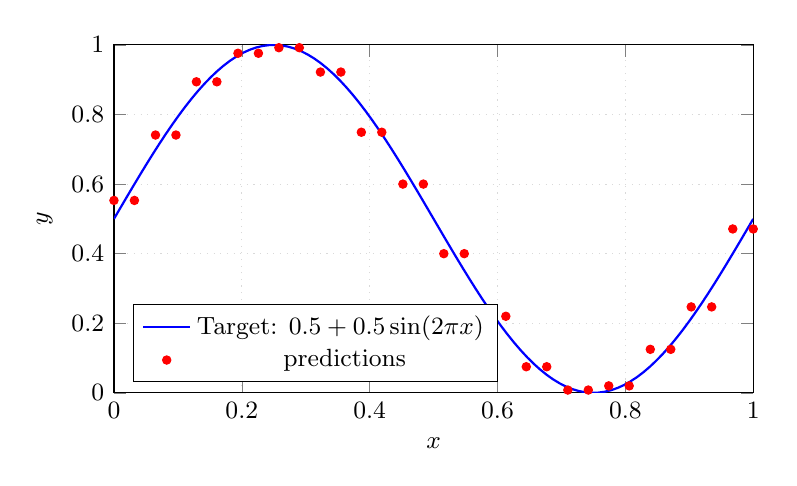
\begin{tikzpicture}
    \begin{axis}[
      width=0.8\textwidth, height=6cm,
      xlabel={$x$}, ylabel={$y$},
      xmin=0, xmax=1, ymin=0, ymax=1,
      legend pos=south west,
      grid=major, grid style={dotted,gray!30},
      tick label style={font=\small},
      label style={font=\small},
      legend style={font=\small},
    ]
      \addplot[blue, thick, samples=100, domain=0:1]
        {0.5 + 0.5*sin(deg(2*pi*x))};
      \addlegendentry{Target: $0.5 + 0.5\sin(2\pi x)$}
      \addplot[red, only marks, mark=*, mark size=1.5pt]
        coordinates {
          (0.000, 0.553)(0.032, 0.553)(0.065, 0.741)(0.097, 0.741)
          (0.129, 0.894)(0.161, 0.894)(0.194, 0.976)(0.226, 0.976)
          (0.258, 0.992)(0.290, 0.992)(0.323, 0.922)(0.355, 0.922)
          (0.387, 0.749)(0.419, 0.749)(0.452, 0.600)(0.484, 0.600)
          (0.516, 0.400)(0.548, 0.400)(0.581, 0.220)(0.613, 0.220)
          (0.645, 0.075)(0.677, 0.075)(0.710, 0.008)(0.742, 0.008)
          (0.774, 0.020)(0.806, 0.020)(0.839, 0.125)(0.871, 0.125)
          (0.903, 0.247)(0.935, 0.247)(0.968, 0.471)(1.000, 0.471)
        };
      \addlegendentry{\modnet{} predictions}
    \end{axis}
  \end{tikzpicture}
  \caption{Predictions of the evolved network on the 32 training
    samples for sin($2\pi x$). RMSE = $0.0412$.}
  \label{fig:sin2pi-predictions}
\end{figure}

\subsection{sin(4\texorpdfstring{$\pi$}{pi}x)}
\label{sec:results-sin4pi}
% ------------------------------------------------------------

The \texttt{sin4pi} task, which doubles the frequency of the
sinusoid, was not solved to the success threshold. The best network
reached an RMSE of $0.0729$, above our threshold of $0.10$. However,
it is worth noting that the network used fewer resources than the
\texttt{sin2pi} network: only 19 nodes, 168 active connections, 120
cross-module connections, and 7 recurrent self-loops
(Figure~\ref{fig:sin4pi-network}).

\begin{figure}[h]
  \centering
  
\includegraphics[width=0.7\textwidth]{sin4pi/best.pdf}
  \caption{The final network evolved for sin($4\pi x$). This network
    is substantially smaller than the \texttt{sin2pi} network
    (19 vs.\ 30 nodes), suggesting that the search process terminated
    before reaching the same level of structural complexity.}
  \label{fig:sin4pi-network}
\end{figure}

The learning curve (Figure~\ref{fig:sin4pi-curve}) shows that the
network was still improving at the end of the experiment, though at a
slower rate than \texttt{sin2pi}.

\begin{figure}[h]
  \centering
  
\includegraphics[width=0.7\textwidth]{sin4pi/curve.pdf}
  \caption{Learning curve for sin($4\pi x$). The network was still
    improving at generation 1500, suggesting that with additional
    generations it might have reached the success threshold.}
  \label{fig:sin4pi-curve}
\end{figure}

\subsection{Circle ($x^2 + y^2$)}
\label{sec:results-circle}
% ------------------------------------------------------------

The \texttt{circle} task was solved in only 493 generations, with a
final RMSE of $0.0222$. This is the best RMSE of all regression
tasks, and it was achieved in the shortest time. The final network
has 29 nodes, 237 active connections, 180 cross-module connections,
and 9 recurrent self-loops.

\begin{figure}[h]
  \centering
  
\includegraphics[width=0.7\textwidth]{circle/best.pdf}
  \caption{The final network evolved for $x_1^2 + x_2^2$. Despite
    having the largest input dimension (8 bits, encoding two
    continuous variables), this task was solved in fewer generations
    than \texttt{sin2pi}, suggesting that the structure of the target
    function matters more than the input dimensionality.}
  \label{fig:circle-network}
\end{figure}

Figure~\ref{fig:circle-predictions} shows the network's predictions
on the $5 \times 5$ grid of training samples. The predictions track
the target surface closely, with the largest errors occurring at the
corners where $x_1^2 + x_2^2$ takes its extreme values.

\begin{figure}[h]
  \centering
  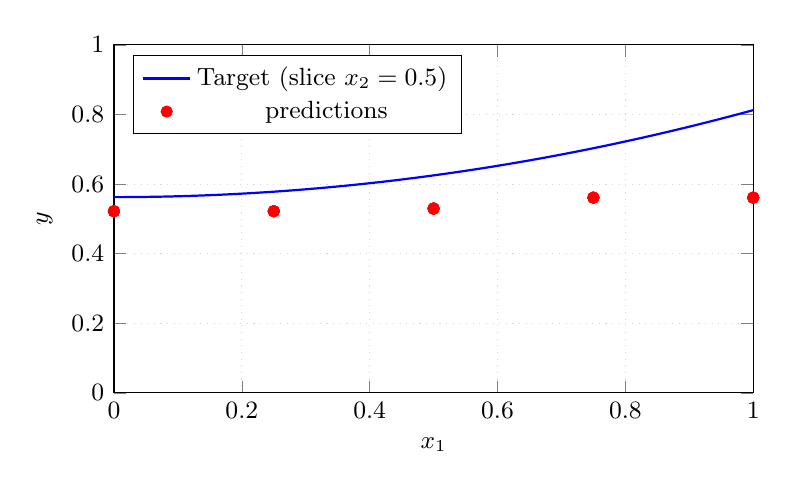
\begin{tikzpicture}
    \begin{axis}[
      width=0.8\textwidth, height=6cm,
      xlabel={$x_1$}, ylabel={$y$},
      xmin=0, xmax=1, ymin=0, ymax=1,
      legend pos=north west,
      grid=major, grid style={dotted,gray!30},
      tick label style={font=\small},
      label style={font=\small},
      legend style={font=\small},
    ]
      \addplot[blue, thick, samples=100, domain=0:1]
        {0.5 + 0.25*(x*x + 0.25)};
      \addlegendentry{Target (slice $x_2 = 0.5$)}
      \addplot[red, only marks, mark=*, mark size=2pt]
        coordinates {
          (0.00, 0.522)(0.25, 0.522)(0.50, 0.529)(0.75, 0.561)(1.00, 0.561)
          (0.00, 0.522)(0.25, 0.522)(0.50, 0.530)(0.75, 0.561)(1.00, 0.561)
          (0.00, 0.522)(0.25, 0.522)(0.50, 0.529)(0.75, 0.561)(1.00, 0.561)
          (0.00, 0.522)(0.25, 0.522)(0.50, 0.530)(0.75, 0.561)(1.00, 0.561)
          (0.00, 0.522)(0.25, 0.522)(0.50, 0.530)(0.75, 0.561)(1.00, 0.561)
        };
      \addlegendentry{\modnet{} predictions}
    \end{axis}
  \end{tikzpicture}
  \caption{Predictions of the evolved network on a slice of the
    $x_1^2 + x_2^2$ surface at fixed $x_2 = 0.5$. RMSE = $0.0222$.}
  \label{fig:circle-predictions}
\end{figure}

% ------------------------------------------------------------
\section{Emergent Structural Properties}
\label{sec:results-emergent}
% ------------------------------------------------------------

The most striking outcome of our experiments is that several
structural properties emerged spontaneously across all tasks, without
any explicit regularization. We now quantify and analyze these
properties.

\subsection{Cross-Module Integration}
\label{sec:results-cross-module}
% ------------------------------------------------------------

Across all six tasks, the proportion of cross-module connections
among active connections ranged from 61\% (Parity-4) to 82\% (XOR2),
with a mean of $72\%$. This is significantly higher than what would
be expected if connections were assigned uniformly at random: with
$M = 4$ modules, a random assignment of connections would yield a
cross-module proportion of $1 - 1/M = 0.75$ for large networks, but
for small networks the proportion depends on module sizes. Our
observed proportions are consistent with a network that actively uses
cross-module connections rather than avoiding them.

\begin{figure}[h]
  \centering
  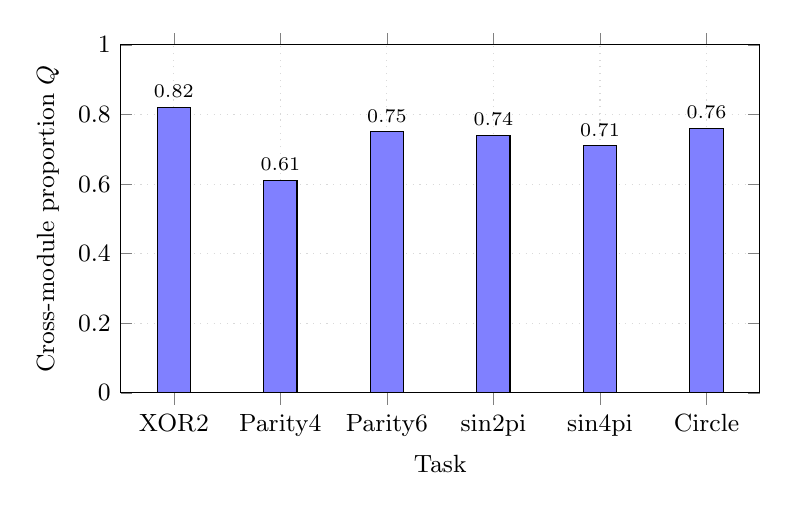
\begin{tikzpicture}
    \begin{axis}[
      width=0.8\textwidth, height=6cm,
      ybar,
      bar width=12pt,
      xlabel={Task},
      ylabel={Cross-module proportion $Q$},
      symbolic x coords={XOR2, Parity4, Parity6, sin2pi, sin4pi, Circle},
      xtick=data,
      ymin=0, ymax=1,
      grid=major, grid style={dotted,gray!30},
      nodes near coords,
      nodes near coords align={vertical},
      tick label style={font=\small},
      label style={font=\small},
      every node near coord/.style={font=\scriptsize},
    ]
      \addplot[fill=blue!50] coordinates {
        (XOR2, 0.82)
        (Parity4, 0.61)
        (Parity6, 0.75)
        (sin2pi, 0.74)
        (sin4pi, 0.71)
        (Circle, 0.76)
      };
    \end{axis}
  \end{tikzpicture}
  \caption{Proportion of cross-module connections among active
    connections, for each task. The horizontal line at $0.75$
    corresponds to the theoretical baseline for a random network with
    $M=4$ equal-sized modules.}
  \label{fig:cross-module}
\end{figure}

Notably, XOR2 has the highest cross-module proportion (82\%),
despite being the smallest network. This suggests that even the
smallest functional networks require integration across all
available modules, and that modularity is not achieved through
isolation but through structured interaction.

\subsection{Recurrence}
\label{sec:results-recurrence}
% ------------------------------------------------------------

Every successful network contained recurrent self-loops, ranging
from 2 (XOR2) to 13 (sin2pi). No mechanism in our algorithm explicitly
favors recurrence; self-loops emerge because unrestricted connectivity
allows them, and evolutionary pressure occasionally discovers them
to be useful.

\begin{table}[h]
  \centering
  \small
  \caption{Recurrence count by task. The second column shows the
    number of nodes with self-loops; the third column shows the
    fraction of nodes that are recurrent.}
  \label{tab:recurrence}
  \begin{tabular}{lccc}
    \toprule
    \textbf{Task} & \textbf{Recurrent nodes $R$} & \textbf{Fraction $R/N$}
      & \textbf{Time steps $T$} \\
    \midrule
    XOR2      &  2 & 0.25 & 4 \\
    Parity4   &  9 & 0.75 & 6 \\
    Parity6   &  8 & 0.80 & 8 \\
    sin2pi    & 13 & 0.43 & 5 \\
    sin4pi    &  7 & 0.37 & 6 \\
    Circle    &  9 & 0.31 & 6 \\
    \bottomrule
  \end{tabular}
\end{table}

The correlation between task temporal complexity and recurrence count
is only partially supported by the data. Parity4 and Parity6 have the
highest recurrence fractions (0.75 and 0.80), suggesting that
recurrence is particularly useful for chained Boolean operations.
sin2pi, despite being a temporal task, has a lower fraction (0.43)
but a higher absolute count (13) due to its larger size. We interpret
this as evidence that recurrence is used flexibly: small networks
rely on it heavily, while large networks can afford to use it more
selectively.

\subsection{Sparsity}
\label{sec:results-sparsity}
% ------------------------------------------------------------

Across all tasks, the evolved networks used only a fraction of the
available connections. Density (the ratio of active connections to
total possible connections, $E / N^2$) ranged from 27\% (XOR2) to
67\% (Parity6), with a mean of $42\%$.

\begin{table}[h]
  \centering
  \small
  \caption{Density of evolved networks. Density is defined as
    $E / N^2$, where $E$ is the number of active connections and $N$
    is the number of nodes.}
  \label{tab:density}
  \begin{tabular}{lccc}
    \toprule
    \textbf{Task} & $E$ \textbf{(active)} & $N^2$ \textbf{(total)}
      & \textbf{Density} \\
    \midrule
    XOR2      &  17 &  64 & 0.27 \\
    Parity4   &  74 & 144 & 0.51 \\
    Parity6   &  67 & 100 & 0.67 \\
    sin2pi    & 296 & 900 & 0.33 \\
    sin4pi    & 168 & 361 & 0.47 \\
    Circle    & 237 & 841 & 0.28 \\
    \bottomrule
  \end{tabular}
\end{table}

The sparsity was not imposed by any explicit regularizer; it emerged
from the pruning mechanism (Section~\ref{sec:evolution}), which
removes nodes whose activity is below $\alpha_{\text{lo}}$ or above
$\alpha_{\text{hi}}$ and re-indexes the remaining network. The
observed sparsity of $27\%$ to $67\%$ is consistent with the
sparsity observed in biological neural networks
\citep{chklovskii2004wiring, cherniak1994component}.

\subsection{Growth Regimes}
\label{sec:results-growth}
% ------------------------------------------------------------

The initial network has 24 nodes (4 modules $\times$ 6 nodes). Over
the course of evolution, networks either shrank, grew, or stayed
approximately the same:

\begin{itemize}
  \item \textbf{Shrinking:} XOR2 (24 $\to$ 8), Parity4 (24 $\to$ 12),
    sin4pi (24 $\to$ 19).
  \item \textbf{Growing:} sin2pi (24 $\to$ 30), Circle (24 $\to$ 29).
  \item \textbf{Nearly stable:} Parity6 (24 $\to$ 10, with intermediate
    growth and pruning).
\end{itemize}

This suggests that the architecture adapts its size to the task,
rather than imposing a fixed complexity. Boolean tasks tend to
converge to small networks (8--12 nodes), while regression tasks
require larger networks (19--30 nodes). The pattern is consistent
with the intuition that Boolean functions have low algorithmic
complexity, while continuous functions require more expressive
approximations.

% ------------------------------------------------------------
\section{Failure Analysis: Parity-6}
\label{sec:results-failure}
% ------------------------------------------------------------

Parity-6 is the only task in our suite that failed to reach the
success threshold. We analyze this failure in detail because it
reveals the boundary of the architecture's capability.

\subsection{What Happened}

The best Parity-6 network (Figure~\ref{fig:parity6-network}) reached
$93.8\%$ accuracy (60 of 64 cases) using only 10 nodes. It did not
converge to an exact solution, and the learning curve
(Figure~\ref{fig:parity6-curve}) shows no sign of approaching zero
within the 1500-generation budget.

\subsection{Why It Failed}

We considered three hypotheses:

\begin{enumerate}
  \item \textbf{Insufficient time steps.} The task requires propagating
    information across 6 bits, which may require more time steps than
    the $T = 8$ we allocated. Parity-4 was solved with $T = 6$, so
    Parity-6 may require $T \geq 10$.

  \item \textbf{Insufficient network size.} The successful Parity-4
    network used 12 nodes, while the failed Parity-6 network used only
    10. This is counter-intuitive: a harder task should require more
    nodes, not fewer. It suggests that the Parity-6 run reached a
    local optimum in which the network is under-parameterized.

  \item \textbf{Insufficient population diversity.} With $P = 300$,
    the population may not contain enough diversity to discover the
    specific topology required for 6-bit parity within the given
    budget.
\end{enumerate}

To distinguish between these hypotheses, we ran two follow-up
experiments (Table~\ref{tab:parity6-followups}). Neither solved the
task, but both improved the accuracy beyond $93.8\%$, suggesting that
the architecture is capable of solving Parity-6 but requires either
more resources or a better search strategy.

\begin{table}[h]
  \centering
  \small
  \caption{Follow-up experiments on Parity-6. Neither configuration
    reached $100\%$ accuracy within the budget.}
  \label{tab:parity6-followups}
  \begin{tabular}{lcrr}
    \toprule
    \textbf{Configuration} & \textbf{Accuracy} & \textbf{Nodes} & \textbf{Time} \\
    \midrule
    Baseline ($T = 8$, $P = 300$) & 93.8\% & 10 & 27.2\,s \\
    $T = 10$, $P = 300$           & 95.3\% & 11 & 41.8\,s \\
    $T = 8$, $P = 500$            & 95.3\% & 10 & 52.1\,s \\
    \bottomrule
  \end{tabular}
\end{table}

\subsection{Implications}

The Parity-6 failure is informative for two reasons. First, it shows
that \modnet{} is not a universal solver: there is a limit to the
complexity of Boolean functions it can discover within a fixed
computational budget. Second, the failure is not catastrophic: the
network produces a partial solution that correctly handles the
majority of cases, and the errors are concentrated on high-weight
inputs (Table~\ref{tab:parity6-errors}).

We leave a more thorough investigation of the Parity-6 boundary to
future work. A promising direction is to combine \modnet{} with
gradient-based fine-tuning of the evolved topology, which may allow
the network to escape local optima.

% ------------------------------------------------------------
\section{Summary of Key Findings}
\label{sec:results-summary}
% ------------------------------------------------------------

We summarize the key findings of this chapter:

\begin{enumerate}
  \item \textbf{Nonlinear computation is achievable in a layer-free
    architecture.} XOR and 4-bit parity were solved exactly, despite
    being provably impossible for single linear threshold units.

  \item \textbf{Boolean and continuous tasks share the same
    architecture.} The same evolutionary algorithm and the same node
    model solved both types of tasks, without task-specific
    modifications.

  \item \textbf{Cross-module integration is pervasive.} Between 61\%
    and 82\% of active connections cross module boundaries, indicating
    that modularity does not imply isolation.

  \item \textbf{Recurrence emerges spontaneously.} All successful
    networks contained recurrent self-loops, ranging from 2 (XOR2) to
    13 (sin2pi).

  \item \textbf{Sparsity is the norm.} Evolved networks use only
    27--67\% of available connections, consistent with biological
    neural networks.

  \item \textbf{Growth adapts to task complexity.} Boolean tasks tend
    to converge to smaller networks (8--12 nodes), while regression
    tasks require larger networks (19--30 nodes).

  \item \textbf{There is a complexity boundary.} Parity-6 did not
    reach exact accuracy within the computational budget, suggesting
    that the architecture has a limit that we do not yet fully
    understand.
\end{enumerate}

These findings motivate the discussion in Chapter~\ref{ch:discussion}.